\chapter{Results}

In this chapter the main results of the numerical investigation of the Bose-Hubbard superfluid to Mott-insulator phase transition are presented.

The framework set up for performing optimal control of lattice systems consist of multiple components working together:\\
The quantum state of the system is parametrized as a Matrix Product State (see Chapter \ref{chap:MPS}), whereby the exponential scaling of the Hilbert space with system size can be avoided. For time evolving the state a version of the tDMRG algorithm is employed (see Section \ref{sec:modTMDRG}), which is modified to accommodate some of the difficulties otherwise associated with the control problem.
Quantum optimal control determines the best way to manipulate a set of external parameters in order to facilitate a state transfer $\ket{\psi_0} \to \ket{\psi_{\mathrm{target}}}$. These states are calculated initially using the DMRG algorithm (see Section \ref{sec:DMRG}) at the fixed control points $\boldsymbol{u}(0)$ and $\boldsymbol{u}(T)$, such that these states are guaranteed to be the ground state. Most of the tensor operations used are implemented in the ITensor library \cite{ITensor}.
The optimal set of control parameters needed for completing the state transfer with the highest possible fidelity is calculated using the GROUP algorithm described in Section \ref{sec:GROUP}. In each iteration of GROUP, the gradient of the cost functional is calculated and used to update the control through the Interior Point method (see Section \ref{sec:IntPoint}). The Interior Point method is implemented in IPOPT library \cite{Wachter2006}.\\

In section \ref{sec:5partOptimization} the optimal control framework is tested on a small lattice of 5 sites in order to gauge the dynamics of the system and determine optimal values of various parameters.\\
The results from conducting optimal control of 20-site lattice with unit occupancy can be found in section \ref{sec:20partOptimization}. 



\section{Characterization of Methods on a Small System} \label{sec:5partOptimization}
To determine the optimal parameters and settings for the optimization, an initial analysis of a small system consisting of 5 sites with unit occupancy was made. Systems of different sizes are expected to evolve differently, especially due to the closed boundary conditions of the lattice, which have a greater impact for smaller systems. Although the dynamics are expected to very with the lattice length, certain parameters such as the regularization factor, $\gamma$, and the dimension of the chopped basis, $M$, can optimized using a smaller system. These parameters only affect the shape of the control pulse, which is subjected to constraints independent of the system size. Nevertheless, the optimal value of these parameters may change slightly with system size, since the shape of the optimal control pulse varies both with system size and optimization method used, as shown in \cite{MajaJulie}. 


\subsection{Boundary Conditions}
Section \ref{sec:BHmodel} describes how the Bose-Hubbard model is only well defined within the tight-binding limit. This is especially an issue for lattice depth below the limit, as the Wannier functions may start overlapping with the next-nearest neighbouring sites, thus facilitating two-site hopping, which is not accounted for in the model. Thus, the starting value of the control must be chosen with care. In \cite{FrankBloch,Doria2011} initial lattice depths at $V_0 (0) = 3 E_r$ and lower were chosen, where it was argued that the model is still a decent approximation at this depth. Hence, an initial control of $U/J (0) = 2$ was chosen, which corresponds to a lattice depth around three recoil energies. In order to ensure the validity of the model, the minimum value of the control, which is enforced at all times during the pulse sequence, was set to the same value as the initial control.  
The final control was set to $U/J (T) = 50$ roughly corresponding to the final lattice depth of $V_0 (T) = 14 E_r$ used in \cite{FrankBloch}.\\
The initial and target state were calculated from the control parameter at the start and end of the duration respectively using the DMRG algorithm. Thus, the states are insured to be the ground state at each end of the duration, whereby the optimized state transfer will bring the system in the ground state after the control sequence.


\subsection{Seed Selection}
The success of an optimization process is often dependent on the quality of the initial starting point or seed. Poor seeding strategies can lead to failure in finding optimal solutions when conducting local searches in complex optimization landscapes \cite{Sorensen2016}. This has been demonstrated to occur in constrained quantum control problems \cite{Zhdanov2015}, which is exactly the type of problem examined in this thesis. Hence, the type of seed used for the optimization must be chosen carefully.\\ 
Different adiabatic lattice ramps from the superfluid to Mott-insulator phase were examined in \cite{Zakrzewski2009}. The study concluded that ramping the lattice slowly around the point of the phase transition results in an improved final fidelity. This is very similar to an avoided crossing in a two-level system, $\{ \ket{1} , \ket{2} \}$, due to an external perturbation. In this scenario $\ket{1}$ is the ground state in one asymptotic limit of the external parameter, while $\ket{2}$ is the ground state in the other limit. A transfer $\ket{1} \to \ket{2}$ while remaining in the ground state can be achieved by adiabatically sweeping over the external parameter, whereas a rapid change in this external parameter will result in the final state being excited.\\
Thus, a ramp sequence was proposed in \cite{Zakrzewski2009}, which has an initial sigmoid shape followed by a slow increase in the lattice depth around the phase transition point. Following this, the lattice follows an exponential ramp to its final depth. Examining other attempts of optimizing the ramp sequence of the Bose-Hubbard model \cite{Doria2011,FrankBloch} shows similar traits in their results. Therefore, choosing seeds with a slow ramp across the point of the phase transition followed by a rapid increase in lattice depth should yield good optimization results.
\begin{figure}[h!]
    \centering
    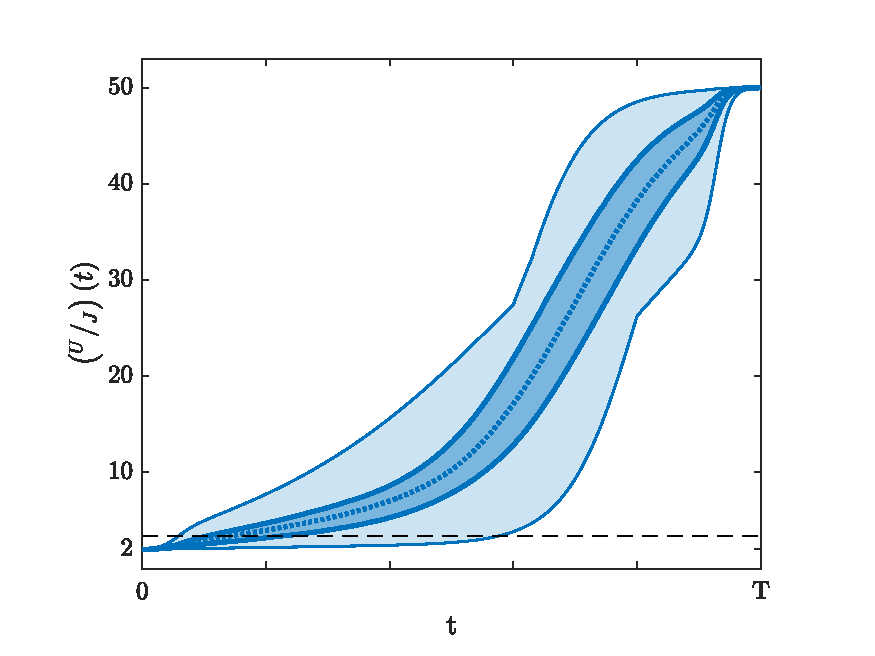
\includegraphics[width=0.7\textwidth]{Figures/LinSigSeed.pdf}
    \caption{\textit{Distribution of seeds used for optimization. All seeds lie within the lightly shaded region, while the darker region contains the 25-75 percentile of seeds. Lastly, the dotted line is the median value of the seed. The dashed line signifies the point of the Bose-Hubbard phase transition.}}
    \label{fig:LinSigSeed}
\end{figure}
Figure \ref{fig:LinSigSeed} shows the distribution of seeds used for the optimizations. Due to control parameter being the interaction strength of the Bose-Hubbard model, the phase transition occurs at quite a low value compared to the final value. Hence, the initial part of the seed is a slowly increasing linear ramp, which crosses the point of the phase transition with a small slope. A shape function has been multiplied to the seeds enforcing a horizontal slope at the start and end of the duration. This helps avoiding any kinks in the control curve, as the optimized part of the control is subjected to a shape function itself.


\subsection{Determining the Quantum Speed Limit}
To understand how the solutions are affected by the duration of the control sequence, a series of optimizations were made while scanning over the duration $T$. For this a regularization factor of $\gamma = 10^{-6}$ was used, while an optimization space dimension of $M = 20$ was used. Since the control is parametrized using a linear combination of smooth functions, the effect of the regularization term is limited, however, it does help the optimization algorithm avoid greatly varying controls during its initial iterations. Lastly, a time-step of $\Delta t = 10^{-2}$ was chosen as a compromise between accuracy and runtime.\\
Figure \ref{fig:FidelityDuration5} shows the final fidelities obtained for various durations from 100 different initial controls.
\begin{figure}[h!]
    \centering
    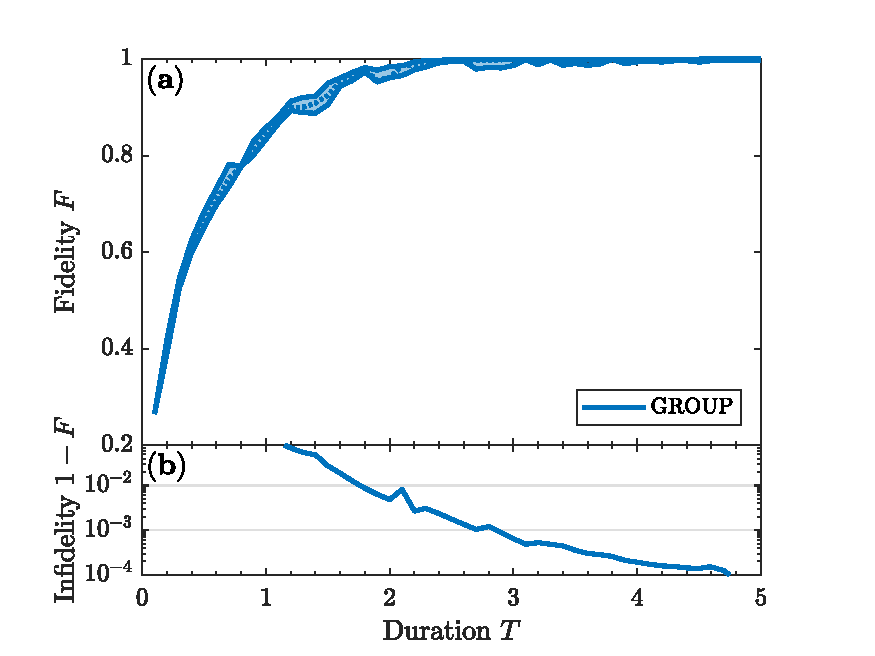
\includegraphics[width=0.8\textwidth]{Figures/5part/FidelityDuration.pdf}
    \caption{\textit{Final fidelity obtained for optimal control at various durations. \textbf{(a)} the dotted line marks the median fidelity achieved, while the shaded area displays the $25\%$- and $75\%$-quartiles of the solutions. \textbf{(b)} the lowest infidelity achieved for each duration. }}
    \label{fig:FidelityDuration5}
\end{figure}
In part \ref{fig:FidelityDuration5}.a the $25\%$- and $75\%$-quartiles along with the median of the solutions are displayed. At short durations the system can not evolve fast enough from the initial state to reach the target state, hence only low fidelities are obtained. However, as more and more time becomes available, fidelities very close to unit can be reached. Although the final fidelity does not appear to improve beyond $T=3$, figure \ref{fig:FidelityDuration5}.b reveals the best solutions still improving at longer durations albeit at a reduced rate.\\
Compared to other figures of merit, the fidelity is a very strong measure, as it only considers the overlap with the target state. Due to the large number of quantum states in lattice systems, achieving unit fidelity is practically impossible, and even reaching a high fidelities become increasingly difficult with system size. An alternative figure of merit was used for the optimal control of a Bose-Hubbard system presented in \cite{FrankBloch}. Instead of determining the convergence through the infidelity, a rescaled variance of the particle numbers in each of the central cites was used. This figure of merit is much less sensitive to the system size, however, it does have some less favorable properties: First, multiple particle configurations different from unit occupancy of each site can achieve a vanishing particle number variance. Furthermore, the preferred state of a single particle on each lattice site is not necessarily the ground state at the final control value, although it is a fairly good approximation. Hence the fidelity is a much better figure of merit, as it provides flexibility with regards to which state is steered towards, and it considers solely the overlap with that exact state.\\
Thus, to determine the quantum speed limit a threshold for accepted final fidelity must be agreed on. This threshold must be variable with the systems size, due to the sensitivity of the fidelity. In \cite{MajaJulie} a similar optimization was made, and an infidelity threshold of $I_{\mathrm{QSL}} = 10^{-3}$ was set for a 3-site lattice. Adopting the same threshold for the results shown in figure \ref{fig:FidelityDuration5} yields a quantum speed limit of $T_{\mathrm{QSL}}^{(5)} = 2.7$.\\

Further information regarding the control landscape as well as the consistency of the algorithm can be inferred from the spread in fidelities shown in figure \ref{fig:FidelityDuration5}.a. A large variety of final fidelities may be due to a control landscape with many local minima. On the other hand, the same phenomenon could be caused by the inability of an algorithm to accurately converge to the minimum. The interior point method is a very robust algorithm capable of handling non-linear constraints, whereby it is reasonable to assume the variations in solutions being caused by the underlying control landscape. Considering the fairly large variation in seeds shown in figure \ref{fig:LinSigSeed}, the control landscape of the 5-site problem must be relatively simple.


\subsubsection{Optimized Ramp Sequences}
A central question is how the optimized ramp sequence differs from its initial seed in both shape and fidelity reached. From figure \ref{fig:FidelityDuration5} one observes that durations around $T = 2.5$ consistently produce solutions with very high fidelity. The lowest infidelities reached at this duration are around $I \approx 10^{-3}$, whereby they are of very high quality. 
\begin{figure}[h!]
    \centering
    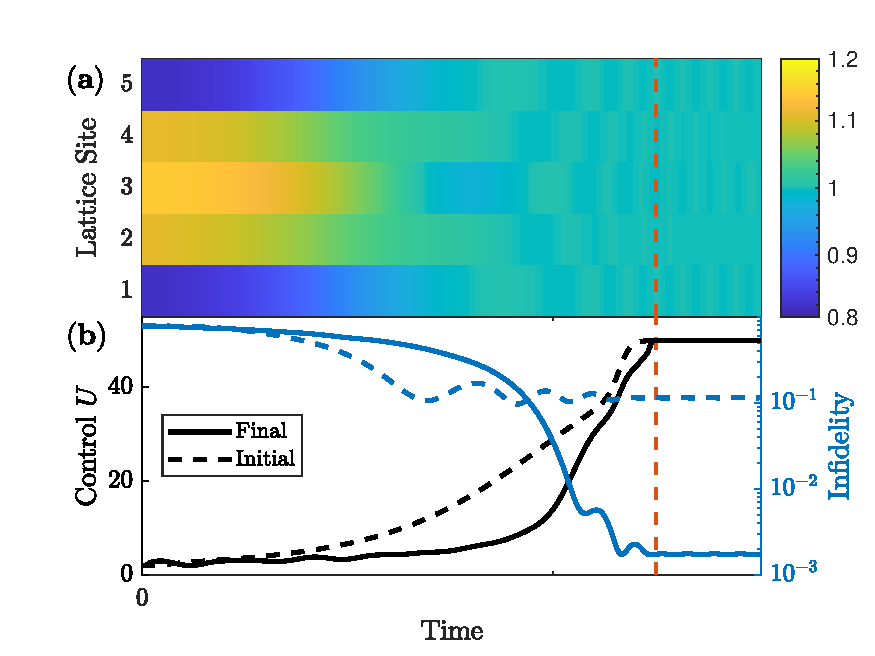
\includegraphics[width=0.8\textwidth]{Figures/5part/ExtendedRampT25.pdf}
    \caption{\textit{Solution with highest fidelity achieved for duration $T = 2.5$. The dashed, red line marks the end of the duration, from which the system is further evolved using the final control value. \textbf{(a)} logarithmically scaled expectation value of the number operator, $\braket{\hat{n}_i}$, for each site as the system is evolved according to the optimized ramp. \textbf{(b)} the initial and optimized ramp sequences along with the corresponding evolution of fidelities.}}
    \label{fig:ExtendedRamp5}
\end{figure}
Figure \ref{fig:ExtendedRamp5} displays the optimized ramp sequence at duration $T = 2.5$ along with an illustration of the evolution of the system. First, consider part \ref{fig:ExtendedRamp5}.b in which the initial and optimized control is plotted together with the resulting infidelity. Optimizing the initial seed utilizing the GROUP algorithm has resulted in an increase of two magnitudes in the final fidelity achieved.
While the initial ramp is fairly smooth, the optimized ramp wiggles a bit during the first half of the duration followed by a sharp upswing towards the final control value. The steep increase in the control towards the end is very similar to the adiabatic ramp sequence proposed in \cite{Zakrzewski2009}, however, the initial oscillating behavior seen in the optimized ramp is very non-adiabatic. In fact, examining the optimized ramp sequences for durations shorter than $T = 2.5$ shows an increase in the amplitude of the ramp oscillations, as solutions are required to be increasingly non-adiabatic in order to reach a good fidelity within the given duration. In the other end of the spectrum, solutions for durations longer than $T = 2.5$ become increasingly adiabatic. Examples of solutions at various durations can be found in Appendix ???.\\
After the given optimization duration the final control value is kept constant for an additional time span, where the system is further evolved. Any residual evolution of the system at this point is due to the system not being an eigenstate of the Hamiltonian corresponding to final control value. When examining the initial and final ramp sequence after the optimization duration, the initial control appears to reach a more stable state. However, this is an illusion caused by the logarithmic axis, as the optimized ramp produces a state much closer to the target state, which is set as the ground state of $\hat{H}(U(T))$ through the DMRG algorithm.\\ 
Figure \ref{fig:ExtendedRamp5}.a illustrates the expectation value of the number operator, $\braket{\hat{n}_i}$, for each site during the ramp. Initially the system is in the superfluid state causing a low energetic cost for having multiple particles on each sites. Thus, one observes a reduced number of particles at the outer sites of the lattice due to the closed boundary conditions. As the system is evolved towards the Mott-Insulating state, having multiple particles at the same sites becomes very unfavorable energetically. Hence, the target state has a single particle at each site, as it is deep in the Mott regime. The optimized ramp brings the system very close to this configuration of particles, however, some imperfections are present although their magnitude is exaggerated by the logarithmic color axis. The residual oscillations of the infidelity after the optimization durations can be seen in figure \ref{fig:ExtendedRamp5}.a as fluctuations of the particle number. 


\subsubsection{Control Basis Size}
Unlike GRAPE, which takes the full optimization space into account, parametrizations like GROUP utilize a chopped basis resulting in a much smaller dimension of the optimization space. When reducing the dimension of the optimization space through a parametrization as described in eq. \eqref{eq:controlParametrization}, the new control basis must be able to span the solution space. Otherwise artificial minima can be introduced to the control landscape due to the incompleteness of the basis \cite{Rach2015}. 
In the implementation of GROUP used for these calculations, the basis functions of the chopped basis are $f_n = \sin \left( \omega_n t / T \right)$, where $\omega_n = n \pi$. These functions also constitute the complete set eigenfunctions for the quantum mechanical problem of a particle trapped in a one-dimensional, infinitely deep well. Similarly, the control value is bounded by a constant upper and lower limit, whereby the full sine-basis is capable of describing all solutions. However, in the chopped basis only the $M$ lowest frequencies are used for the parametrization.
To investigate the basis size required to describe the optimal solutions, a series of optimizations were made for various basis sizes at the duration $T = 2.5$. 
\begin{figure}[h!]
    \centering
    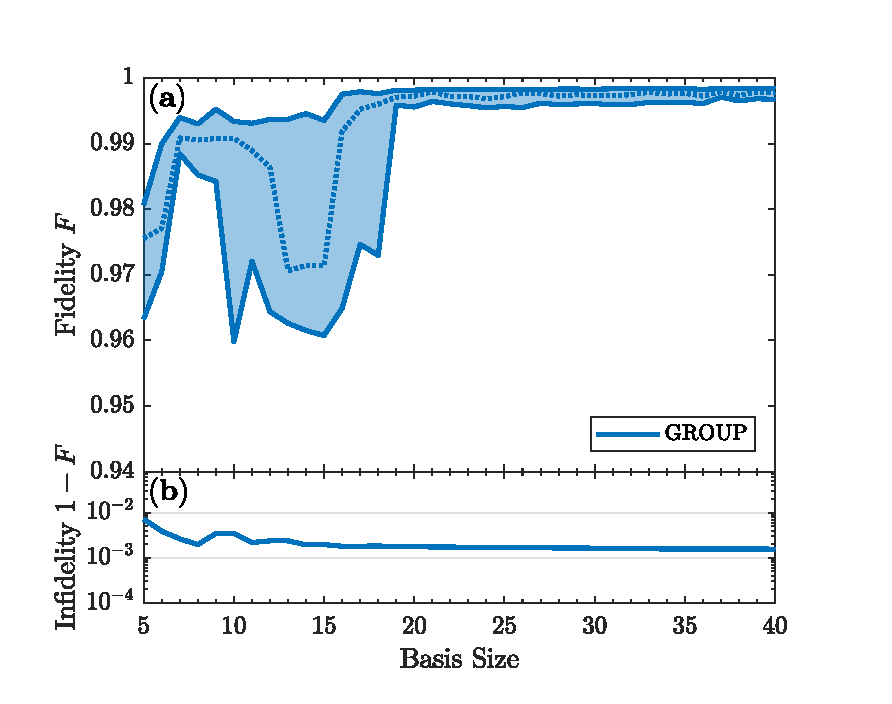
\includegraphics[width=0.8\textwidth]{Figures/5part/BestFidelityBasisSize.pdf}
    \caption{\textit{Final fidelity obtained for optimal control at various optimization space dimensions for duration $T = 2.5$. \textbf{(a)} the dotted line marks the median fidelity achieved, while the shaded area displays the $25\%$- and $75\%$-quartiles of the solutions. \textbf{(b)} the lowest infidelities achieved for each basis size.}}
    \label{fig:FidelityBasisSize5}
\end{figure}
The results of the scan over the basis size can be seen in figure \ref{fig:FidelityBasisSize5}. From figure \ref{fig:FidelityBasisSize5}.a it is evident that a basis size of around 20 and above consistently produces high-fidelity solutions, while the quality of solutions using a smaller basis size fluctuated greatly. Thus, high-fidelity ramps for $T = 2.5$, as the one previously shown in figure \ref{fig:ExtendedRamp5}, have at least 20 frequency components. Although results obtained with a smaller basis are generally worse due to the reduced optimization space causing artificial minima, high fidelity solutions are still possible to achieve, as the optimal solution may still be realizable using only few frequencies. This can be observed in figure \ref{fig:FidelityBasisSize5}.b, where the infidelity of the best solution remains constant, while the overall fidelity of the solutions converged to decreases. Thus, a large spread in final fidelity is a consequence of a more complicated optimization landscape causing the interior point method to converge to non-optimal points.


\section{Optimal Control of Large Lattice Systems} \label{sec:20partOptimization}